\documentclass[12pt]{article}
\usepackage{sbc-template}
\usepackage{graphicx,url}
\usepackage[brazil]{babel}   
\usepackage[utf8]{inputenc}  
\sloppy

\title{Android Things - A metamorfose de um sistema operacional}

\author{Nobre Junior, E. J. R.\inst{1}}


\address{Universidade Estadual de Santa Cruz (UESC)\\ 
  Campus Soane Nazaré de Andrade, Rodovia Jorge Amado, Km 16, Bairro Salobrinho\\45662-900 -- Ilhéus - BA - Brazil 
  \email{eduardo.reisnobre@gmail.com}
}

\begin{document} 

\maketitle

\begin{abstract}
	The subject of Internet of Things is no longer only occupied by embedded Linux-based systems in simpler constructions, opening a market for more robust and powerful systems. This article aims to present the reasons and means by which Android Things, an operating system made for the internet environment of things came to exist, as well as under what bases it was built and what changes and differences it presents when compared to its bases.
\end{abstract}
     
\begin{resumo} 
	O assunto de Internet das Coisas vem deixando de ser ocupado apenas por sistemas embarcados baseados em Linux em construções mais simplórias, passando a abrir um mercado para sistemas mais robustos e poderosos. Esse artigo busca apresentar os motivos e meios pelos quais o Android Things, um sistema operacional feito para o ambiente de internet das coisas passou a existir, assim como sob quais bases ele foi construído e quais alterações e diferenças ele apresenta quando comparado com suas bases.
\end{resumo}


\section{Introdução}
Tendo o início de seu desenvolvimento lançamento em 23  de setembro de 2008 o Android OS, um produto desenvolvido com direção da Google em parceria com as empresas HTC, Sony, Intel, Motorola, Qualcomm, Dell, Texas Instruments, Samsung Electronics, LG Electronics, T-Mobile e outras sob o consórcio conhecido como OHA (Open Handset Alliance), sendo um projeto de código aberto que hoje domina 76.53\% do mercado de sistemas operacionais móveis \cite{statcounter}
vem passando por diversas mudanças em suas estruturas básicas buscando mais velocidade, segurança ou visando atingir uma fatia maior do mercado. Através do projeto com o codinome Brillo o android evoluiu e se transformou para atender uma nova demanda de mercado causada pela ubiquidade da internet na sociedade moderna dando origem em maio de 2018 ao Android Things, uma plataforma desenvolvida para a internet da coisas.
\section{IoT}
A criação do Android Things se deu quando uma sugestão do impensável foi feita. Sistemas embarcados vinham sendo feitos com o uso de distribuições linux, até que a sugestão de uma versão do Android, capaz de funcionar sem interface, algo impensável em um sistema operacional no qual a forma primária de interação se dá através de uma tela.
\\Apesar das dificuldades, as vantagens como reaproveitamento de bases de código assim como mão de obra foram argumentos fortes o suficiente para dar início ao que um dia se tornaria o Android Things.
\\Através do projeto Brillo, o Android passou a poder existir sem uma interface com um tamanho até 10\% do tamanho original e com alterações no launcher padrão do Android e a redução nos serviços dos quais o Android depende. A seção a seguir explica as características das arquiteturas assim como suas diferenças.

\section{Arquitetura} \label{sec:firstpage}
\subsection{Android}
O sistema operacional Android em sua arquitetura é composto de cinco grandes camadas com suas características e propriedades únicas. 
\begin{figure}[ht]
\centering
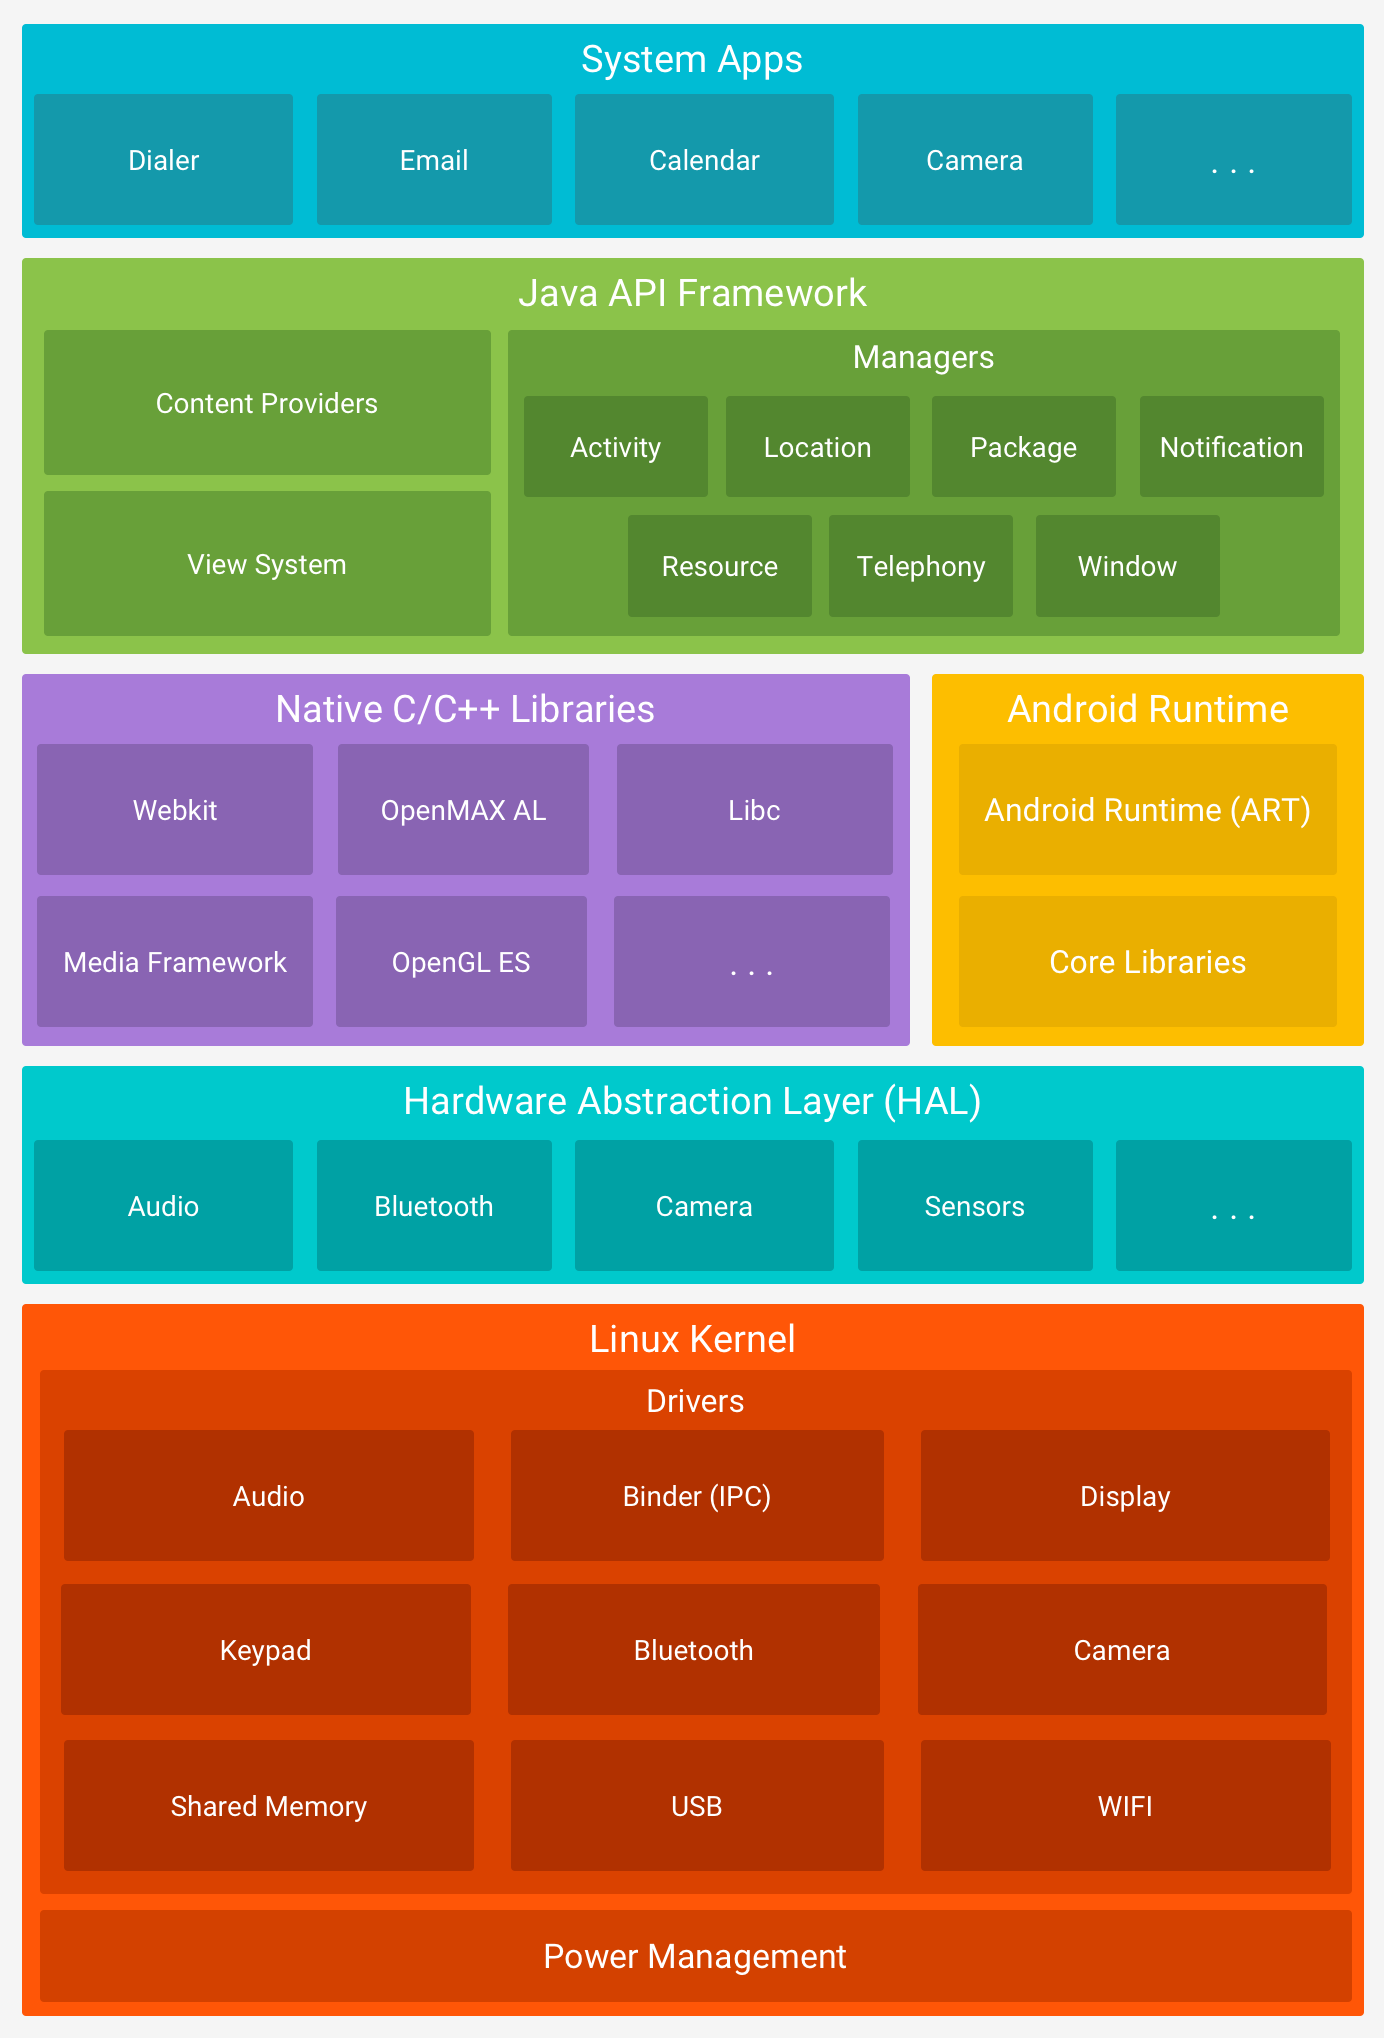
\includegraphics[width=.6\textwidth]{images/android-stack_2x.png}
\caption{The Android software stack}
\captionsource{\textbf{Fonte:}}{\cite{developer:platform}}
\label{fig:androidstack}
\end{figure}

\\A primeira camada (System Apps) contém serviços básicos da google como SMS, calendários, navegadores e outros. Aplicações existentes na instalação do sistema operacional não possuem prioridade. Ao se instalar uma aplicação de terceiros, esta pode se tornar o novo padrão para o sistema operacional \cite{developer:platform}.
\\A segunda camada (Java Api Framework) como o nome indica, contém as API’s fornecidas pela linguagem Java. Essa camada existe para permitir a reutilização dos componentes internos.
\\Essa camada incluí:
\begin{itemize}
	\item um sistema de views para construção de interfaces,
	\item um gerenciador de recursos, responsável por pelo acesso a conteúdos estáticos, como bitmaps, definições de layouts e afins,
	\item um gerenciador de notificações, que além de ser responsável por notificações do sistema, fornece uma api para outras aplicações construírem notificações,
	\item Um gerenciador de atividades, sendo a base para construção de todos os aplicativos na plataforma Android fornecendo rotinas de ciclos de vidas e servindo como ponto de entrada interações do usuário, assim como fornece comportamentos padrões para todos os aplicativos, como o uso do botão back,
	\item Provedores de conteúdos, que fornecem uma interface para aplicações acessarem dados armazenados por si mesmos ou por outros aplicativos. Encapsulando os dados ele garante segurança através desse mecanismo, assim como garante um padrão que conecta dados de um processo a outros.
\end{itemize}
A terceira camada contém as bibliotecas padrões das quais partes centrais do sistema como o Android Runtime e o Hardware Abstraction Layer dependem. A plataforma expõe funcionalidades dessas bibliotecas através do Android Framework.
\\A quarta camada, Android Runtime (ART), incluído nas versões superiores a 5 em substituição a máquina virtual \textbf{Dalvik}, permite que cada aplicação seja executada como um processo independente. ART é construído para executar múltiplas máquinas virtuais, incluindo: 
\begin{itemize}
	\item compilações no estilo Ahead-of-time (AOT) e just-in-time (JIT)
	\item Garbage Collection (GC) otimizada
	\item Melhor suporte a debug.
\end{itemize}
A quinta camada serve como interface entre o alto nível e o baixo nível, expondo as funcionalidades do hardware através da API do Java Framework. É constituída de múltiplos módulos para realizar a interface com uma funcionalidade em questão, como a câmera ou bluetooth do seu dispositivo.
\\A sexta e última é a base do sistema operacional em si, o Kernel do Linux. O ART depende do kernel do Linux para realizar operações com threads e gerenciamento de memória em baixos níveis. Essa camada fornece drivers para várias áreas de controle de hardware como áudio, display, bluetooth, câmera. Além dos drivers o kernel do Linux garante uma interface para gerenciamento de energia.

\subsection{Android Things}
Esse sistema operacional é baseado diretamente na API 7.0 (Nougat) do android citada acima com algumas modificações.
\begin{figure}[ht]
\centering
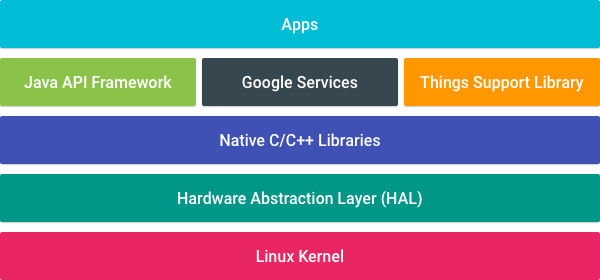
\includegraphics[width=.6\textwidth]{images/platform-architecture.png}
\caption{Android Things Stack}
\captionsource{\textbf{Fonte:}}{\cite{developer:platform}}
\label{fig:androidstack}
\end{figure}

A primeira camada contém as aplicações padrões do sistema operacional, assim como as aplicações de terceiros.
\\A segunda camada, onde a API do Java Framework existe, é bem similar a utilizada no Android citada acima onde displays (barra de status e barras de navegação) são opcionais na sua versão headless.
\\A terceira camada é composta por serviços do Google, implementados nativamente, a lista de serviços é extensa e contém desde integrações com Firebase que é lida com todo back-end de aplicações, assim como Cast, uma tecnologia da google utilizada nos dispositivos ChromeCast e na linha de produtos Google Home.
\\A quarta camada, Things Support Library, lida com a comunicação entre dispositivos e drivers. Através de Interfaces Java, o sistema operacional fornece APIs para controle de sensores, atuadores e afins através de diversos protocolos padrões como:
\begin{itemize}
	\item GPIO
	\item I2C
	\item PWM
	\item SPI
	\item UART
\end{itemize}
As duas últimas camadas são comparáveis em componentes e função às encontradas no Android, portanto não há a necessidade de explorá-las nesta seção.

\section{Modelo de Programação}
O modelo de programação utilizado atualmente atual utilizado faz uso do Renderscript introduzido na versão 3.0 do Android \cite{apache}. Essa alteração foi  feita para resolver problemas de performance existentes nos modelos SDK e NDK anteriormente utilizados. Tendo como base a linguagem C99 que se refere ao padrão ISO/IEC 9899/1999 \cite{wiki:c99} e introduz outros padrões de programação. A idéia central desse modelo de programação é compilar o código para uma representação intermediária próxima da arquitetura alvo. A aplicação então é empacotada e distribuída com uma representação intermediária e o runtime engine compila essa representação em instruções de máquina.
\\O código fonte em Renderscript é compilado para dois targets: LLVM bitcode como uma representação imediata do programa e um reflexo das classes Java como uma camada de interface entre o código Android SDK e o código do Renderscript.
\\\\As definições acima lidam com definições gerais sobre o estilo de código e tecnologias, porém ao se codificar aplicações o programador deve estar ciente dos chamados blocos base que são Classes Java fazem parte do Java API Framework e que são os padrões de comunicação que todas as aplicações devem utilizar, para por exemplo, enviar uma notificação e afins. Esses blocos bases são Activities, Managers e Services.
\subsection{Activities}
\textbf{Activity} é uma Classe básica que fornece eventos de ciclo de vida para seus objetos assim como funcionam como ponto de entrada para que um usuário interaja com sua aplicação. Para realizar interface com um sensor por exemplo, uma atividade é utilizada como base para protocolos de comunicação e comportamentos padrões comuns entre todos os sensores. 
\\Normalmente atividades são chamadas explicitamente, ao se chamar uma função, porém, ao se utilizar Intent filters é possível chamar atividades implicitamente. Temos uma chamada explícita onde a atividade pode ser “Desligue a luz da sala 01”, porém uma chamada implícita pode ter o seguinte formato “Desligue as luzes” o sistema vai, baseado em uma dada lógica da aplicação, que pode se basear em, através de qual microfone o comando está sendo dado, desligar as luzes no cômodo onde o usuário se encontra.
\subsection{Outros conceitos}
Outros conceitos importantes são os Managers e Services. Managers são utilizados para se se acessar capacidades de hardware como bluetooth, câmeras e afins. 
\\Services são utilizados para operações na nuvem, como o uso da API do Google Maps e outras.
\section{Modelo de Execução}
No centro do modelo de execução se encontra o Android runtime (ART), que é um ambiente de tempo de execução usado pelo sistema operacional. Introduzindo compilação ahead-of-time, o ART compila as aplicações em tempo de instalação para código de máquina. A introdução de um novo modelo de execução, em substituição da máquina virtual Dalvik foi feita mantendo a retrocompatibilidade pois ART utiliza o mesmo estilo de bytecodes através de arquivos .dex como parte dos arquivos contidos nos arquivos de saída .apk.
\\Com o uso de Renderscript a aplicação divide-se em uma parte de alto nível e uma de baixo nível. A primeira parte é o código desenvolvido com o uso do SDK e é responsável pelas funções de suporte como gerenciamento de recursos, ciclo de vida de atividades, a segunda parte é o código Renderscript de baixo nível escrito em C99 e é onde a maioria das funcionalidades das aplicações se encontram, assim como a parte gráfica.
\section{Uso de Recursos}
Nem todos os processos possuem a mesma prioridade em um sistema operacional. Em implementações de IoT certas ações precisam ser tratadas com maior prioridade, para evitar tais problemas o sistema operacional tende a priorizar aplicações com as quais o usuário está interagindo. Em sistemas IoT padrões isso tende a não ser uma preocupação muito grande, já que poucas tarefas são realizadas por um mesmo sistema operacional, em contrapartida, o Android Things tende a ser algo mais completo e integrado onde um mesmo sistema operacional tende a realizar múltiplas tarefas como por exemplo, monitorar a temperatura e realizar o controle de uma unidade de ar condicionado no background enquanto o sistema responde a uma solicitação feita no Google Home para acender lâmpadas em uma sala. Situações como essas são comuns onde uma das tarefas sendo realizadas pelo sistema operacional tem uma maior prioridade do que a outra.
\\\\Dispositivos Android utilizam o algoritmo de Completely Fair Queuing (CFQ) \cite{wiki:cfq} para entradas e saídas de disco, o algoritmo coloca as requisições submetidas pelos processos em um número de filas por processo e aloca fatias de tempo para cada fila. A duração da fatia dependendo da prioridade de entrada e saída da fila. CFQ deve garantir uma alocação justa para todas as aplicações em execução e garantindo uma melhor na taxa de transferência em geral.
\subsection{Prioridade de Processos}
A quantidade de tempo dedicada a uma tarefa normalmente está diretamente ligada a sua prioridade. No exemplo anterior, a captura dos resultados dos sensores possuem uma menor prioridade em relação a resposta necessária para o usuário. Todos os processos são criados com uma prioridade. Desenvolvedores podem definir explicitamente a prioridade de um processo baseado nos requerimentos da aplicação. É possível realizar a alteração do alteração da prioridade durante a execução.
\subsection{Grupos de Controle do Linux Kernel}
O sistema operacional faz extenso uso de grupos de controle para gerenciamento de atividades. Grupos de controle é uma parte do Linux Kernel que permite agregar uma coleção de aplicações e seus futuros processos filhos e threads em grupos hierarquizados \cite{martin}, criando restrições comuns para conjuntos de processos. Esses grupos podem ser utilizados para limitar uso de recursos, prioridades e afins. Em android Cgroups são são utilizados para gerenciar as prioridades das aplicações em primeiro plano.
\section{Conclusão}
Podemos ver através desse artigo as vantagens do uso de uma arquitetura em camadas, onde cada parte move-se individualmente, trazendo um nível de flexibilidade impossível em aplicações monolíticas. O Android Things, apesar de ser uma ferramenta ainda em crescimento, por ser baseado em bases sólidas como o Kernel do Linux e o Android 7.0 Nougat vem trazendo para o campo do IoT uma nova visão de sistemas embarcados.

\bibliographystyle{sbc}
\bibliography{sbc-template}

\end{document}
